\subsection{Kuroda Transformation}

Wie bereits erkl\"art st\"osst man bei der  Umsetzung  in Mikrostreifentechnik
auf  problemen.  Mithilfe  der  Kuroda-Transformation   werden  problematische
Leitungsst\"ucke umgewandelt. In einem ersten Schritt werden beidseitig je ein
Einheitselement  U.E.  mit  der  Eingangswellenimpedanz  $Z  =  \SI{50}{\ohm}$
angeh\"angt.  Diese Elemente ver\"andern  die  D\"ampfungsfunktion  nicht.  In
einem   zweiten   Schritt   werden  diese  U.E.  ``\"uber  die  Induktivit\"at
geschoben''.   Dabei  wird  die  Induktivit\"at  zur  Kapazit\"at,   und   die
Wellenimpedanz des U.E. wird ver\"andert.

Wegen der Symmetrie der g-Parameter in unserem Beispiel k\"onnen die U.E. auch
nur von einer Seite  des  Filters bis in die Mitte hineingeschoben werden, und
nach  der Transformation k\"onnen die resultierende  Wellenimpedanzen  einfach
gespiegelt werden.

Die resultierenden Wellenimpedanzen sind hier aufgelistet.

\begin{align*}
    Z_0  &= \SI{50}{\ohm}    & Z_6  &= \SI{115.8}{\ohm} \\
    Z_1  &= \SI{137.4}{\ohm} & Z_7  &= \SI{26.22}{\ohm} \\
    Z_2  &= \SI{78.62}{\ohm} & Z_8  &= \SI{78.62}{\ohm} \\
    Z_3  &= \SI{26.22}{\ohm} & Z_9  &= \SI{137.4}{\ohm} \\
    Z_4  &= \SI{115.8}{\ohm} & Z_10 &= \SI{50   }{\ohm} \\
    Z_5  &= \SI{20.15}{\ohm} &      &                   \\
\end{align*}

In der Abbildung \ref{fig:stripline-kuroda} Schaltung des Filters gezeigt. Bei
einem  Tiefpass n-ter Ordnung w\"aren $n -  1$  Einheitselemente  n\"otig,  um
s\"amtliche  Induktivit\"aten  in  Kapazit\"aten  zu   transformieren.   Dabei
k\"onnten auch alle U.E. von einer  Seite  in das Filter geschoben werden oder
beidseitig symmetrisch.

In  der  Abbildung  \ref{fig:graph-kuroda}  ist  der  Amplitudengang  und  die
Reflexion  zu  sehen.  Vergleicht  man  sie  mit   dem   Verhalten   vor   der
Kuroda-Transformation (Abbildung \ref{fig:graph-richards}), so wird man keinen
Unterschied  feststellen  k\"onnen;  sie verhalten sich genau gleich (bis  auf
eine lineare Phasenverschiebung).

Damit ist das Filter nun auch Realisierbar, weil die  Stubs  jetzt  geometrish
getrennt  sind  und  nicht  mehr  wie  vorher  alle  am  gleichen  Ort  waren.

\begin{figure}[h!]
    \centering
    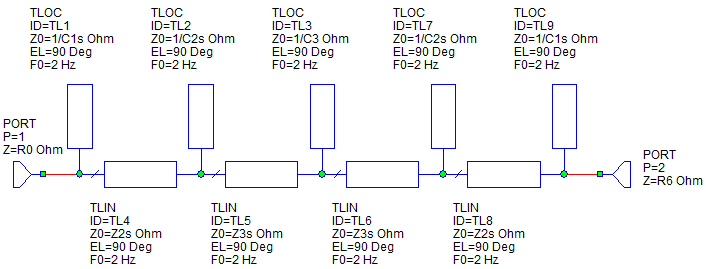
\includegraphics[width=\imagewidth]{images/stripline-kuroda}
    \caption{Resultierende Umwandlung der Schaltung mithilfe der Kuroda-Transformation}
    \label{fig:stripline-kuroda}
\end{figure}

\begin{figure}[h!]
    \centering
    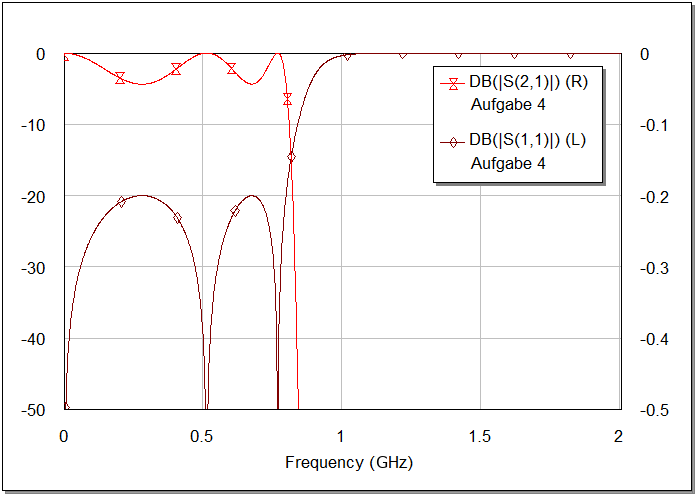
\includegraphics[width=\imagewidth]{images/graph-kuroda}
    \caption{}
    \label{fig:graph-kuroda}
\end{figure}


\subsubsection{Realisierbarkeit}

Es  sollte  noch  angemerkt werden, dass  Leitungsfilter  nur  in  einem  sehr
eingeschr\"ankten Bereich realisierbar sind.  LC-Filter  sind  im  Bereich von
$10^6:1$  sehr gut  realisierbar,  aber  bei  Mikrowellenschaltungen  ist  der
verf\"ugbare Bereich sehr eingeschr\"ankt.

\begin{figure}[h!]
    \centering
    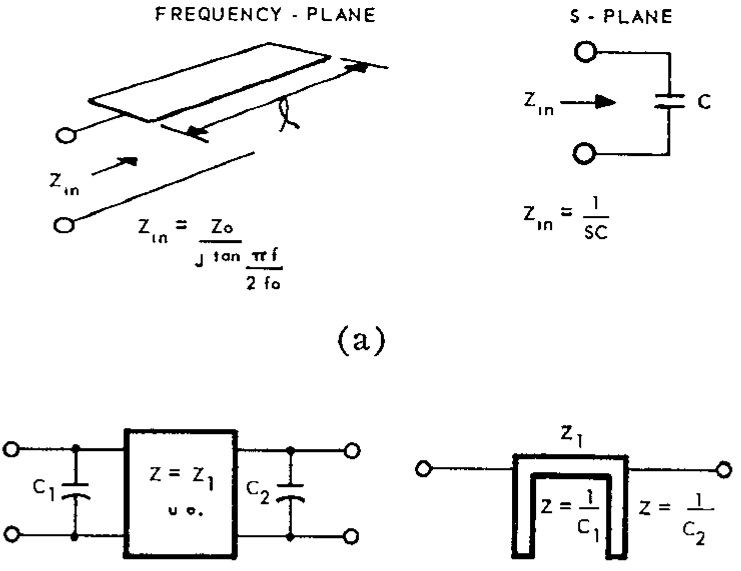
\includegraphics[width=\imagewidth]{images/bereich}
    \caption{Auszug aus \cite{ref:wenzel}: (a) Realisierung einer Kapazit\"at als Stichleitung, (b) Netzwerk in der S-Ebene, (c) Realisierung der Stichleitung}
    \label{fig:bereich}
\end{figure}

Betrachtet  man als Beispiel  ein  einfaches  TEM-Netzwerk  einer  Kapazit\"at
(siehe Abbildung \ref{fig:bereich}), sieht man, dass die  Wellenimpedanz $Z_0$
von  der Kapazit\"at $\frac{1}{C}$ abh\"angt. W\"urde man  die  Wellenimpedanz
$Z_0$ in Funktion der L\"ange $l$ plotten, so w\"urde man schnell feststellen,
dass f\"ur $Z_0<10$ die Leitungsst\"ucke sehr breit werden und  f\"ur  $Z_0  >
300$ die Leitungsst\"ucke sehr schmal werden.

Der Umsetzbare Bereich von $Z_0$ und  somit  von  $C$  ist  also  nur  in  der
Gr\"ossenordnung von $1:30$.

